

\begin{center}
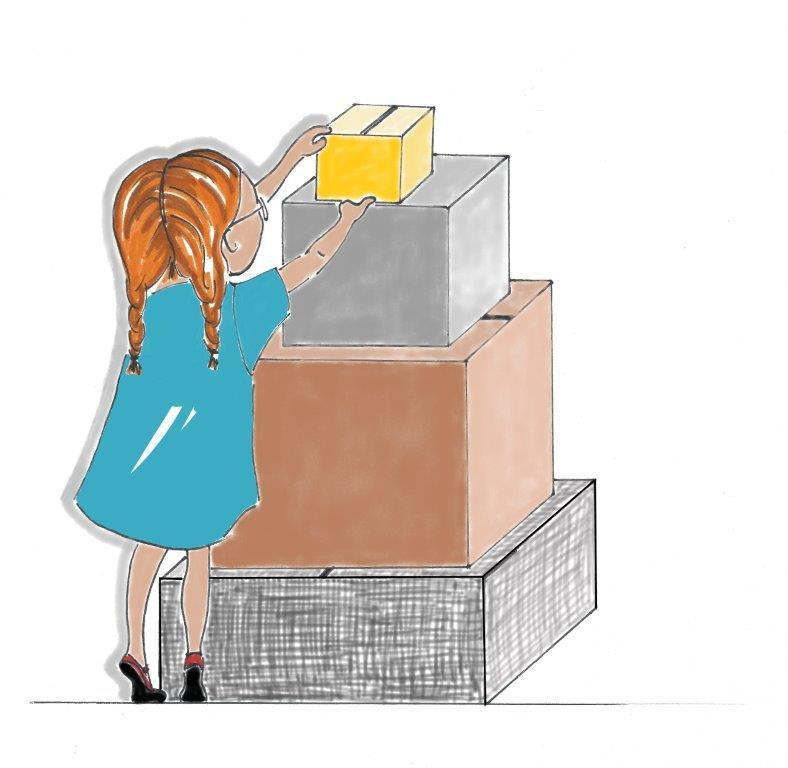
\includegraphics[width=0.6\textwidth]{content/3/chapter4/images/11.png}\\
Cippi prepares the packages
\end{center}

Modules are one of the four big features of C++20: concepts, modules, ranges, and coroutines. Modules promise a lot: shorter compile times, macro isolation, abolishing header files, and avoiding ugly workarounds. Before I present the advantages of modules, I want to step back and explain their benefits.

\subsubsubsection{4.2.1\hspace{0.2cm} Why do we need Modules?}

Let me start with a simple executable. For obvious reasons, I create a helloWorld.cpp program.

\hspace*{\fill} \\ %插入空行
\noindent
A simple hello world program
\begin{lstlisting}[style=styleCXX]
// helloWorld.cpp

#include <iostream>

int main() {
	std::cout << "Hello World" << '\n';
}
\end{lstlisting}

Making an executable helloWorld out of the program helloWorld.cpp with \href{http://gcc.gnu.org/}{GCC} increases its size by factor 130.

\begin{center}
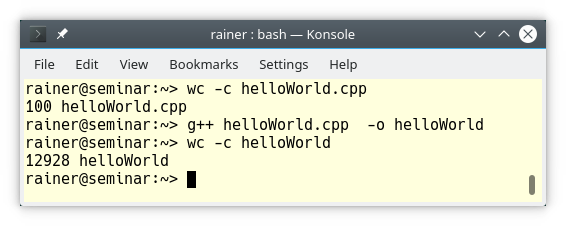
\includegraphics[width=0.8\textwidth]{content/3/chapter4/images/12.png}\\
Size of an object file
\end{center}

The numbers 100 and 12928 in the screenshot stand for the number of bytes. Okay. We should have a basic understanding of what’s happening under the hood.

\hspace*{\fill} \\ %插入空行
\noindent
4.2.1.1\hspace{0.2cm} The Classical Build Process

The build process consists of three steps: preprocessing, compilation, and linking.

\hspace*{\fill} \\ %插入空行
\noindent
4.2.1.1.1\hspace{0.2cm} Preprocessing

The preprocessor handles the directives as \#include and \#define. The preprocessor substitutes \#include directives with the corresponding header files, and it substitutes the macros (\#define). Thanks to directives such as \#if, \#else, \#elif, \#ifdef, \#ifndef, and \#endif parts of the source code can be included or excluded.

This straightforward text substitution process can be observed by using the compiler flag -E on GCC/Clang, or /E on Windows.

\begin{center}
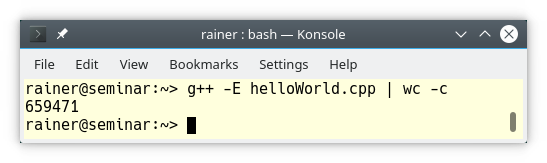
\includegraphics[width=0.8\textwidth]{content/3/chapter4/images/13.png}\\
Preprocessors output
\end{center}

WOW!!! The output of the preprocessing step has more than half a million bytes. I don’t want to blame GCC, the other compilers are similarly verbose. The output of the preprocessor is the input for the compiler.

The result of this preprocessing step is the translation unit.

\hspace*{\fill} \\ %插入空行
\noindent
4.2.1.1.2\hspace{0.2cm} Compilation

The compilation is performed separately on each output of the preprocessor. The compiler parses the C++ source code and converts it into assembly code. The generated file is called an object file and it contains the compiled code in binary form. The object file can refer to symbols that don’t have a definition. The object files can be put in archives for later reuse. These archives are called static libraries.

The objects files that the compiler produces are the inputs for the linker.

\hspace*{\fill} \\ %插入空行
\noindent
4.2.1.1.3\hspace{0.2cm} Linking

The output of the linker can be an executable or a static or shared library. It’s the job of the linker to resolve the references to undefined symbols. Symbols are defined in object files or in libraries. The typical error in this phase is that symbols aren’t defined or are defined more than once.

This build process that consists of the three steps is inherited from C. It works sufficiently well if you have only one translation unit. But when you have more than one, many issues can occur.

\hspace*{\fill} \\ %插入空行
\noindent
4.2.1.2\hspace{0.2cm} Issues of the Build Process

Here’s an incomplete list of the flaws in a classical build process, which can be overcome with modules.

\hspace*{\fill} \\ %插入空行
\noindent
4.2.1.2.1\hspace{0.2cm} Repeated Substitution

The preprocessor substitutes \#include directives with the corresponding header files. Let me change my initial helloWorld.cpp program to make the repetition visible. I refactored the program and added two source files hello.cpp and world.cpp. The source file hello.cpp provides the function hello and the source file world.cpp provides the function world.

Both source files include the corresponding headers. Refactoring means that the program has the same external behavior such as the previous program helloWorld.cpp, but the internal structure is improved. Here are the new files:

\begin{itemize}
\item 
hello.cpp and hello.h

\noindent
Implementation of hello
\begin{lstlisting}[style=styleCXX]
// hello.cpp

#include "hello.h"

void hello() {
	std::cout << "hello ";
}
\end{lstlisting}

\noindent
Header of hello
\begin{lstlisting}[style=styleCXX]
// hello.h

#include <iostream>

void hello();
\end{lstlisting}

\item 
world.cpp and world.h

\noindent
Implementation of world
\begin{lstlisting}[style=styleCXX]
// world.cpp

#include "world.h"

void world() {
	std::cout << "world";
}
\end{lstlisting}

\noindent
Header of world
\begin{lstlisting}[style=styleCXX]
// world.h

#include <iostream>

void world();
\end{lstlisting}

\item 
helloWorld2.cpp

\noindent
Use of hello and world
\begin{lstlisting}[style=styleCXX]
// helloWorld2.cpp

#include <iostream>

#include "hello.h"
#include "world.h"

int main() {
	
	hello();
	world();
	std::cout << '\n';
}
\end{lstlisting}


\end{itemize}

Building and executing the program works as expected:

\begin{center}
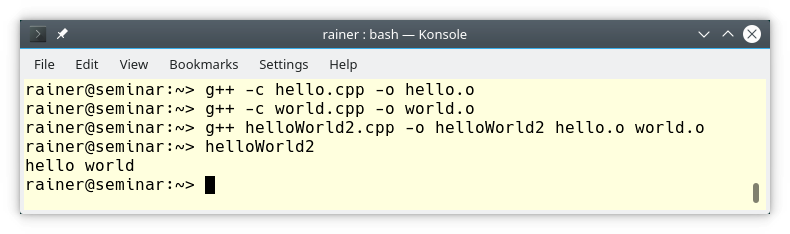
\includegraphics[width=0.8\textwidth]{content/3/chapter4/images/14.png}\\
Compilation of a simple program
\end{center}

Here is the issue. The preprocessor runs on each source file. This means that the header file <iostream> is included a total of three times. Consequently, each source file is blown up to more than half a million lines.

\begin{center}
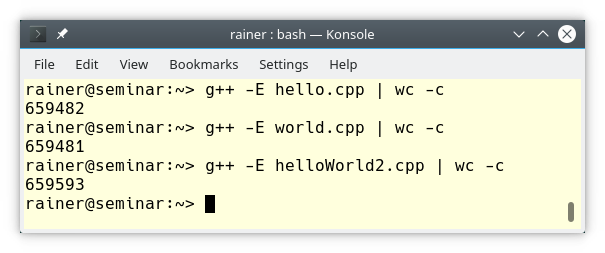
\includegraphics[width=0.8\textwidth]{content/3/chapter4/images/15.png}\\
Size of the preprocessed source file
\end{center}

This is a waste of compile time.

Unlike header files, a module is only imported once and is literally for free.

\hspace*{\fill} \\ %插入空行
\noindent
4.2.1.2.2\hspace{0.2cm} Isolation from Preprocessor Macros

If there is one consensus in the C++ community, it’s the following one: we should get rid of the preprocessor macros. Why? Using a macro is simply text substitution, excluding any C++ semantics. Of course, this has many negative consequences: for example, it may depend on which sequence you include macros, or macros can clash with already defined macros or names in your application.

Imagine you have two header files webcolors.h and productinfo.h.

\hspace*{\fill} \\ %插入空行
\noindent
First definition of macro RED
\begin{lstlisting}[style=styleCXX]
// webcolors.h
#define RED 0xFF0000
\end{lstlisting}

\hspace*{\fill} \\ %插入空行
\noindent
Second definition of macro RED
\begin{lstlisting}[style=styleCXX]
// productinfo.h
#define RED 0
\end{lstlisting}

When a source file client.cpp includes both headers, the value of macro RED depends on the order of the included header. This dependency is very error-prone.

With modules, import order makes no difference.

\hspace*{\fill} \\ %插入空行
\noindent
4.2.1.2.3\hspace{0.2cm} Isolation from Preprocessor Macros

ODR stands for the One Definition Rule and says in the case of a function:

\begin{itemize}
\item 
A function can have not more than one definition in any translation unit.

\item 
A function can not have more than one definition in the program.
\end{itemize}

Inline functions with external linkage can be defined in more than one translation unit. The definitions have to satisfy the requirement that each definition has to be the same.

Let’s see what my linker has to say when I try to link a program breaking the one-definition rule. The following code example has two header files, header.h and header2.h. The main program includes the header files header.h twice and, therefore, breaks the one-definition rule because two definitions of func are included.

\hspace*{\fill} \\ %插入空行
\noindent
Definition of the function func
\begin{lstlisting}[style=styleCXX]
// header.h
void func() {}
\end{lstlisting}

\hspace*{\fill} \\ %插入空行
\noindent
Indirect inclusion of the function definition to func
\begin{lstlisting}[style=styleCXX]
// header2.h
#include "header.h"
\end{lstlisting}

\hspace*{\fill} \\ %插入空行
\noindent
Double definitions of the function func
\begin{lstlisting}[style=styleCXX]
// main.cpp

#include "header.h"
#include "header2.h"

int main() {}
\end{lstlisting}

The linker complains about the multiple definitions of func:

\begin{center}
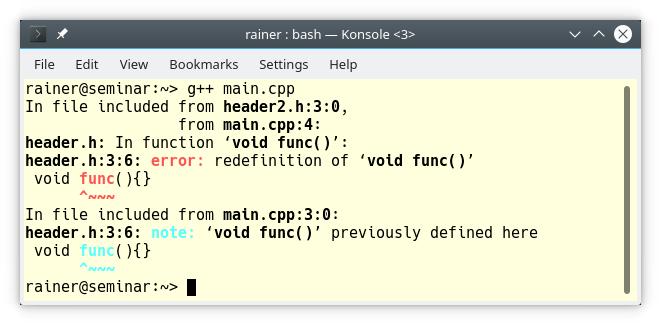
\includegraphics[width=0.8\textwidth]{content/3/chapter4/images/16.png}\\
Breakion the one definition rule
\end{center}

We are used to ugly workarounds, such as putting an include guard around your header. Adding the include guard FUNC\_H to the header file header.h solves the issue.

\hspace*{\fill} \\ %插入空行
\noindent
Using include guards to solve ODR
\begin{lstlisting}[style=styleCXX]
// header.h

#ifndef FUNC_H
#define FUNC_H

void func(){}

#endif
\end{lstlisting}

With modules, duplicate symbols are very unlikely.

I will now summarize the advantages of modules.

\subsubsubsection{4.2.2\hspace{0.2cm} Advantages}

Here are the advantages of modules in a concise form:

\begin{itemize}
\item 
Modules are imported only once and are literally for free.

\item 
It makes no difference in which order you import a module.

\item 
Duplicate symbols with modules are very unlikely.

\item 
Modules enable you to express the logical structure of your code. You can explicitly specify names that should be exported or not. Additionally, you can bundle a few modules into a bigger module and provide them to your customer as a logical package.

\item 
Thanks to modules, there is no need to separate your source code into an interface and an implementation part.
\end{itemize}

\begin{tcolorbox}[colback=blue!5!white,colframe=blue!75!black,title=Regular Types]
Modules in C++ may be older than you think. My short historic detour should give an idea how long it takes to get something so valuable into the C++ standard.

In 2004, Daveed Vandevoorde wrote proposal \href{http://www.open-std.org/jtc1/sc22/wg21/docs/papers/2004/n1736.pdf}{N1736.pdf}, which described for the first time the idea of modules. It took until 2012 to get a dedicated Study Group (SG2, Modules). In 2017, Clang 5.0 and MSVC 19.1 provided the first implementations. One year later, the Modules TS (technical specification) was finalized. Around the same time, Google proposed the so-called ATOM (Another Take On Modules) proposal (\href{http://www.open-std.org/jtc1/sc22/wg21/docs/papers/2018/p0947r1.html}{P0947}) for modules. In 2019, the Modules TS and the ATOM proposal were merged into the C++20 committee draft (\href{https://github.com/cplusplus/draft/releases/tag/n4842}{N4842}).
\end{tcolorbox}

\subsubsubsection{4.2.3\hspace{0.2cm} A First Example}

The purpose of this section is straightforward: I will give you an introduction to modules. More advanced features of modules are in the following sections. Let’s start with a simple math module.

\hspace*{\fill} \\ %插入空行
\noindent
A simple math module
\begin{lstlisting}[style=styleCXX]
// math.ixx

export module math;

export int add(int fir, int sec){
	return fir + sec;
}
\end{lstlisting}

The expression export module math is the module declaration. By putting export before function add’s definition, add is exported and can, therefore, be used by a consumer of the module.

\hspace*{\fill} \\ %插入空行
\noindent
Use of the simple math module
\begin{lstlisting}[style=styleCXX]
// client.cpp

import math;

int main() {
	add(2000, 20);
}
\end{lstlisting}

import math imports module math and makes the exported names in the module visible to client.cpp.

Let me start with the module declaration file.

\hspace*{\fill} \\ %插入空行
\noindent
4.2.3.1\hspace{0.2cm} Module Declaration File

Did you notice the strange name of the module: math.ixx.

\begin{itemize}
\item 
The Microsoft compiler uses the extension ixx. The suffix ixx stands for a module interface source.

\item 
The Clang compiler originally used the extension cppm. The m in the suffix probably stands for module. This convention changes in newer versions of Clang to the cpp extension.

\item 
The GCC compiler uses no special extension.
\end{itemize}

The global module fragment is meant to compose module interfaces. It starts with the keyword module and ends with the module declaration. The global module fragment is the place to use preprocessor directives such as \#include so that the module interface can compile. The code in the global module fragment is not exported by the module interface.

The second version of the module math supports the two functions add and getProduct.

\hspace*{\fill} \\ %插入空行
\noindent
A module definition with a global module fragment
\begin{lstlisting}[style=styleCXX]
// math1.ixx

module;

#include <numeric>
#include <vector>

export module math;

export int add(int fir, int sec){
	return fir + sec;
}

export int getProduct(const std::vector<int>& vec) {
	return std::accumulate(vec.begin(), vec.end(), 1, std::multiplies<int>());
}
\end{lstlisting}

I included the necessary headers between the global module fragment (line 3) and the module declaration (line 8).

\hspace*{\fill} \\ %插入空行
\noindent
Use of the improved module math
\begin{lstlisting}[style=styleCXX]
// client1.cpp

#include <iostream>
#include <vector>

import math;

int main() {
	
	std::cout << '\n';
	
	std::cout << "add(2000, 20): " << add(2000, 20) << '\n';
	
	std::vector<int> myVec{1, 2, 3, 4, 5, 6, 7, 8, 9, 10};
	
	std::cout << "getProduct(myVec): " << getProduct(myVec) << '\n';
	
	std::cout << '\n';
}
\end{lstlisting}

The client imports module math and uses its functionality:

\begin{center}
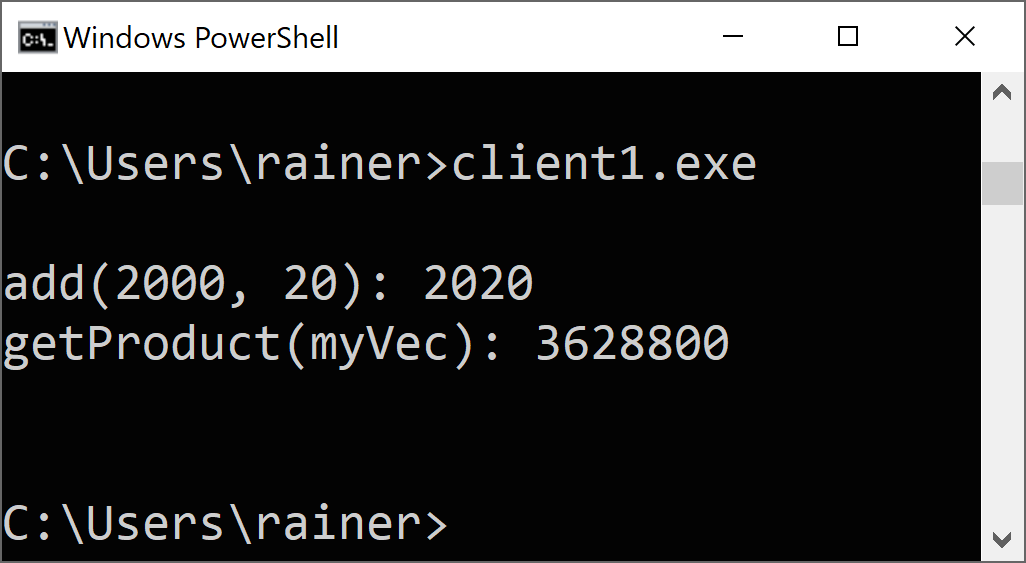
\includegraphics[width=0.5\textwidth]{content/3/chapter4/images/17.png}\\
Execution of the program client1.exe
\end{center}

Now, let’s dive into the details.

\subsubsubsection{4.2.4\hspace{0.2cm} Compilation and Use}

To compile the module math.ixx used by the client program client.cpp, you have to use a very recent Clang, GCC, or Microsoft compiler.

The compilation of a module is challenging. For that reason, I show as an example the compilation of the module with the Microsoft compiler and the Clang compiler.

\hspace*{\fill} \\ %插入空行
\noindent
4.2.4.1\hspace{0.2cm} Microsoft Visual Compiler

First, I use the cl.exe 19.25.28614 for x64 compiler.

\begin{center}
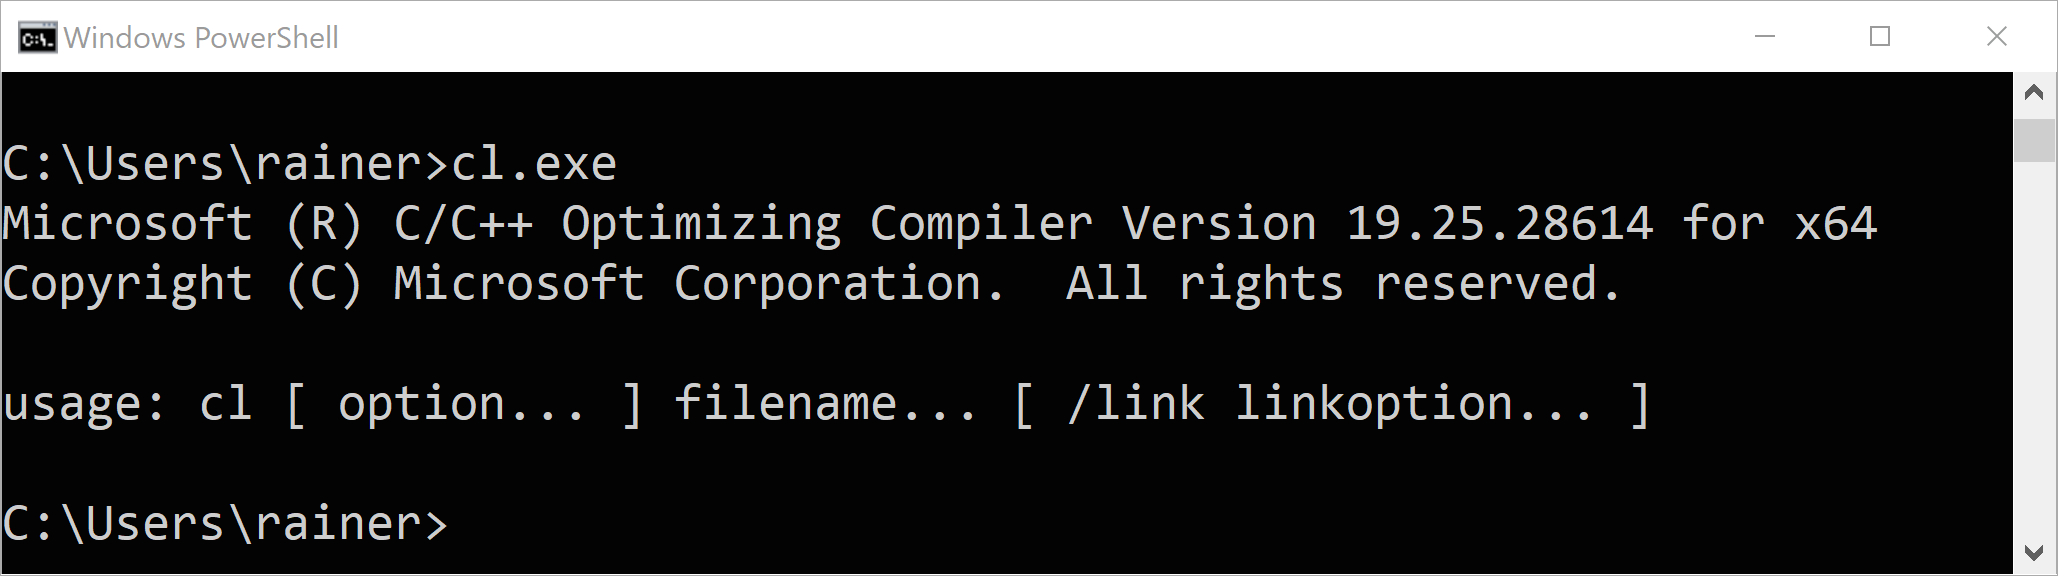
\includegraphics[width=0.8\textwidth]{content/3/chapter4/images/18.png}\\
Microsoft compiler for modules
\end{center}

These are the steps to compile and use the module with the Microsoft compiler. I only show the minimal command line. As promised, more details follow. Additionally, with an older Microsoft compiler, you have to use the flag /std:cpplatest.

\hspace*{\fill} \\ %插入空行
\noindent
Building the executable with the Microsoft compiler
\begin{tcblisting}{commandshell={}}
cl.exe /experimental:module /c math.ixx
cl.exe /experimental:module client.cpp math.obj
\end{tcblisting}

\begin{itemize}
\item 
Line 1 creates an obj file math.obj and an IFC file math.ifc. The IFC file contains the metadata description of the module interface. The binary format of the IFC is modeled after the \href{https://www.stroustrup.com/gdr-bs-macis09.pdf}{Internal Program Representation} by Gabriel Dos Reis and Bjarne Stroustrup (2004/2005).

\item 
Line 2 creates the executable client.exe. Without the implicitly used math.ifc file from the first step, the linker cannot find the module.
\end{itemize}

For obvious reasons, I do not show the output of the program execution.

\hspace*{\fill} \\ %插入空行
\noindent
4.2.4.2\hspace{0.2cm} Clang Compiler

On Linux, I use the Clang 10.0.0 compiler.

\begin{center}
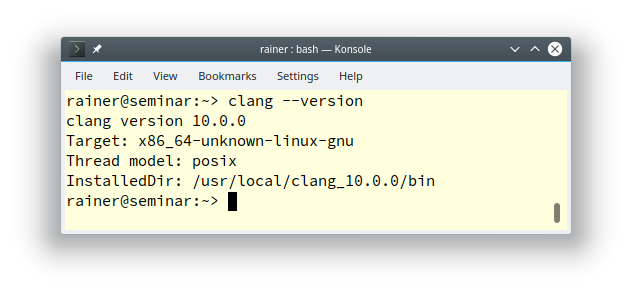
\includegraphics[width=0.8\textwidth]{content/3/chapter4/images/19.png}\\
Clang compiler for modules
\end{center}

With the clang compiler, the module declaration file is simply a cpp file. Consequently, I have to rename the math.ixx file to math.cpp.

\hspace*{\fill} \\ %插入空行
\noindent
A simple math module
\begin{lstlisting}[style=styleCXX]
// math.cpp

export module math;

export int add(int fir, int sec){
	return fir + sec;
}
\end{lstlisting}

The client file client.cpp is unchanged. These are the necessary steps to create the executable.

\hspace*{\fill} \\ %插入空行
\noindent
Building the executable with the Clang compiler
\begin{tcblisting}{commandshell={}}
clang++ -std=c++2a -stdlib=libc++ -c math.cpp -Xclang -emit-module-interface \
   -o math.pcm

clang++ -std=c++2a -stdlib=libc++ -fprebuilt-module-path=. client.cpp math.pcm \
   -o client
\end{tcblisting}

\begin{itemize}
\item 
Line 1 creates the module math.pcm. The suffix pcm stands for precompiled module. The flags -std=c++2a specifies the working draft of the C++20 standard and the -stdlib=libc++ the used C++ standard library. The flag combination -Xclang -emit-module-interface is necessary for creating the precompiled module.

\item 
Line 4 creates the executable client, which uses the module math.pcm. You specify the path to the module with the -fprebuilt-module-path flag.
\end{itemize}

\hspace*{\fill} \\ %插入空行
\noindent
4.2.4.3\hspace{0.2cm} Used Compiler

I use the cl.exe from Microsoft in this book. Microsoft currently has (end 2020) the \href{https://en.cppreference.com/w/cpp/compiler_support}{best support for modules}. The Microsoft blog provides two excellent introductions to modules: \href{https://docs.microsoft.com/en-us/cpp/cpp/modules-cpp?view=msvc-160&viewFallbackFrom=vs-2019}{Overview of modules in C++} and \href{https://devblogs.microsoft.com/cppblog/c-modules-conformance-improvements-with-msvc-in-visual-studio-2019-16-5/}{C++ Modules conformance improvements with MSVC in Visual Studio 2019 16.5}. Neither Clang nor GCC provide similar introductions, making it quite difficult to use modules with those compilers.


\subsubsubsection{4.2.5\hspace{0.2cm} Export}

There are three ways to export names in a module interface unit.

\hspace*{\fill} \\ %插入空行
\noindent
4.2.5.1\hspace{0.2cm} Export Specifier

You can export each name explicitly.

\hspace*{\fill} \\ %插入空行
\noindent
Export specifier
\begin{lstlisting}[style=styleCXX]
export module math;
export int mult(int fir, int sec);
export void doTheMath();
\end{lstlisting}

\hspace*{\fill} \\ %插入空行
\noindent
4.2.5.2\hspace{0.2cm} Export Group

An export group exports all of its names.

\hspace*{\fill} \\ %插入空行
\noindent
Export group
\begin{lstlisting}[style=styleCXX]
export module math;
export {
	int mult(int fir, int sec);
	void doTheMath();
}
\end{lstlisting}

\hspace*{\fill} \\ %插入空行
\noindent
4.2.5.3\hspace{0.2cm} Export Namespace

Instead of an exported group, you can use an exported namespace.

\hspace*{\fill} \\ %插入空行
\noindent
Export namespace
\begin{lstlisting}[style=styleCXX]
export module math;
export namespace math {
	int mult(int fir, int sec);
	void doTheMath();
}
\end{lstlisting}

When a client uses names from an export namespace, they have to qualify those names.

Only names that don’t have an internal linkage can be exported.

\subsubsubsection{4.2.6\hspace{0.2cm} Guidelines for a Module Structure}

Let’s examine guidelines for how to structure a module.

\hspace*{\fill} \\ %插入空行
\noindent
Guidelines for the structure of a module
\begin{lstlisting}[style=styleCXX]
module; // global module fragment
#include <headers for libraries not modularized so far>
export module math; // module declaration; starts the module purview
import <importing of other modules>
<non-exported declarations> // names only visibile inside the module
export namespace math {
	<exported declarations> // exported names
}
\end{lstlisting}

This guideline serves one purpose: give you a simplified structure of a module and also an idea of what I’m going to write about. So, what’s new in this module structure?

\begin{itemize}
\item 
The global module fragment starting with the keyword module is optional. After it and preceding the module declaration is the right place to include headers.

\item 
The module declaration export module math starts the so-called module purview, which ends at the end of the translation unit.

\item 
You can import modules at the beginning of the module purview. The imported modules have module linkage and are not visible outside the module. This observation also applies to the non-exported declarations.

\item 
I put the exported names in namespace math, which has the same name as the module.

\item 
The module has only declared names. Let’s write about the separation of the interface and the implementation of a module.
\end{itemize}

\subsubsubsection{4.2.7\hspace{0.2cm} Module Interface Unit and Module Implementation Unit}

When the module becomes bigger, you should structure it into a module interface unit and one or more module implementation units. Following the previously mentioned guidelines to structure a module, I will refactor the previous version of the math module.

\hspace*{\fill} \\ %插入空行
\noindent
4.2.7.1\hspace{0.2cm} Module Interface Unit

\hspace*{\fill} \\ %插入空行
\noindent
The module interface unit
\begin{lstlisting}[style=styleCXX]
// mathInterfaceUnit.ixx

module;

#include <vector>

export module math;

export namespace math {

	int add(int fir, int sec);
	
	int getProduct(const std::vector<int>& vec);

}
\end{lstlisting}

\begin{itemize}
\item 
The module interface unit contains the exporting module declaration: export module math (line 7).

\item 
The names add and getProduct are exported (lines 11 and 13).

\item 
A module can have only one module interface unit.
\end{itemize}

\hspace*{\fill} \\ %插入空行
\noindent
4.2.7.2\hspace{0.2cm} Module Implementation Unit

\hspace*{\fill} \\ %插入空行
\noindent
The module implementation unit
\begin{lstlisting}[style=styleCXX]
// mathImplementationUnit.cpp

module math;

#include <numeric>

namespace math {

	int add(int fir, int sec) {
		return fir + sec;
	}
	
	int getProduct(const std::vector<int>& vec) {
		return std::accumulate(vec.begin(), vec.end(), 1, std::multiplies<int>());
	}
}
\end{lstlisting}

\begin{itemize}
\item 
The module implementation unit contains non-exporting module declarations: module math; (line 3).

\item 
A module can have more than one module implementation unit.
\end{itemize}

\hspace*{\fill} \\ %插入空行
\noindent
4.2.7.3\hspace{0.2cm} Main Program

\hspace*{\fill} \\ %插入空行
\noindent
The client uses module math
\begin{lstlisting}[style=styleCXX]
// client3.cpp

#include <iostream>
#include <vector>

import math;

int main() {

	std::cout << '\n';
	
	std::cout << "math::add(2000, 20): " << math::add(2000, 20) << '\n';
	
	std::vector<int> myVec{1, 2, 3, 4, 5, 6, 7, 8, 9, 10};
	
	std::cout << "math::getProduct(myVec): " << math::getProduct(myVec) << '\n';
	
	std::cout << '\n';

}
\end{lstlisting}

From the user’s perspective, the module math (line 6) is included and the namespace math was added.

When my explanations become compiler dependent, I put them in a separate tip box. This information is, in general, highly valuable if you want to try it out.


\begin{tcolorbox}[colback=blue!5!white,colframe=blue!75!black,title=Building the Executable with the Microsoft Compiler]
	
Manually building the executable includes a few steps.

\hspace*{\fill} \\ %插入空行
\noindent
Building a module with a module interface unit and a module implementation unit
\begin{tcblisting}{commandshell={}}
cl.exe /c /experimental:module mathInterfaceUnit.ixx /EHsc
cl.exe /c /experimental:module mathImplementationUnit.cpp /EHsc
cl.exe /c /experimental:module client3.cpp /EHsc
cl.exe client3.obj mathInterfaceUnit.obj mathImplementationUnit.obj
\end{tcblisting}

\begin{itemize}
\item 
Line 1 creates the object file mathInterfaceUnit.obj and the module interface file math.ifc.

\item 
Line 2 creates the object file mathImplementationUnit.obj.

\item 
Line 3 creates the object file client3.obj.

\item 
Line 4 creates the executable client3.exe.
\end{itemize}

For the Microsoft compiler, you have to specify the exception handling model (/EHsc), and enable modules: /experimental:module.

Finally, here is the output of the program:

\begin{center}
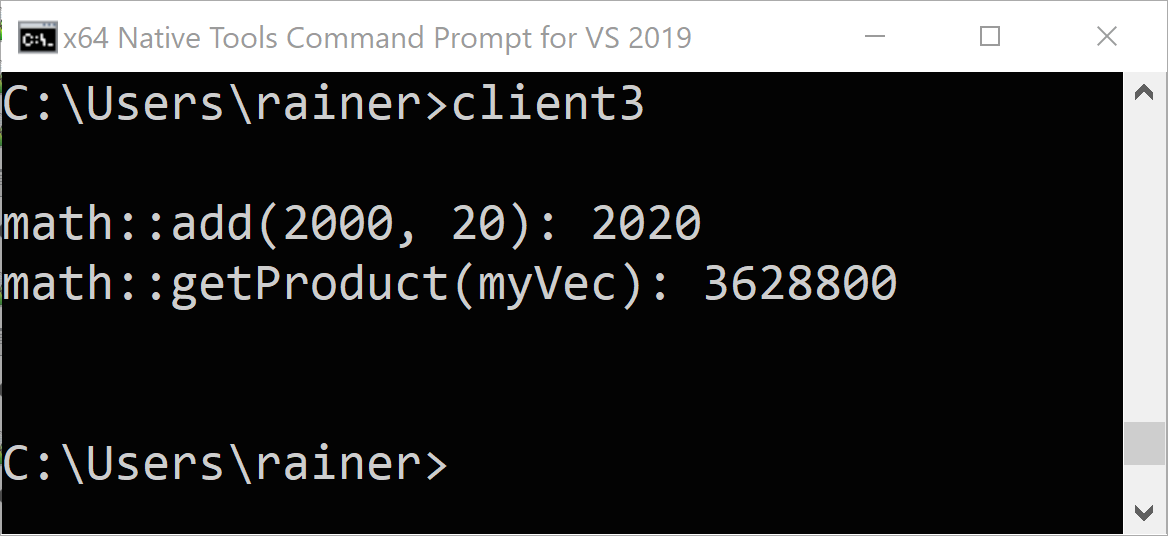
\includegraphics[width=0.6\textwidth]{content/3/chapter4/images/20.png}\\
Execution of the program client2.exe
\end{center}
\end{tcolorbox}

\subsubsubsection{4.2.8\hspace{0.2cm} Submodules and Module Partitions}

When your module becomes bigger, you want to divide its functionality into manageable components. C++20 modules offer two approaches: submodules and partitions.

\hspace*{\fill} \\ %插入空行
\noindent
4.2.8.1\hspace{0.2cm} Submodules

A module can import modules and then re-export them.

In the following example, module math imports the submodules math.math1 and math.math2.

\hspace*{\fill} \\ %插入空行
\noindent
The module math
\begin{lstlisting}[style=styleCXX]
// mathModule.ixx
export module math;
export import math.math1;
export import math.math2;
\end{lstlisting}

The expression export import math.math1 imports module math.math1 and re-exports it as part of the module math.

For completeness, here are the modules math.math1 and math.math2. I used a period to separate the module math from its submodules. This period is not necessary.

\hspace*{\fill} \\ %插入空行
\noindent
The submodule math.math1
\begin{lstlisting}[style=styleCXX]
// mathModule1.ixx
export module math.math1;
export int add(int fir, int sec) {
	return fir + sec;
}
\end{lstlisting}

\hspace*{\fill} \\ %插入空行
\noindent
The submodule math.math2
\begin{lstlisting}[style=styleCXX]
// mathModule2.ixx
export module math.math2;
export {
	int mul(int fir, int sec) {
		return fir * sec;
	}
}
\end{lstlisting}

If you look carefully, you recognize a small difference in the export statements in the modules math. While math.math1uses an export specifier, math.math2 uses an export group or export block.

From the client’s perspective, using the math module is straightforward.

\hspace*{\fill} \\ %插入空行
\noindent
The main program
\begin{lstlisting}[style=styleCXX]
// mathModuleClient.cpp
#include <iostream>
import math;
int main() {
	std::cout << '\n';
	std::cout << "add(3, 4): " << add(3, 4) << '\n';
	std::cout << "mul(3, 4): " << mul(3, 4) << '\n';
}
\end{lstlisting}

Compiling and executing the program gives the expected behavior.

\begin{center}
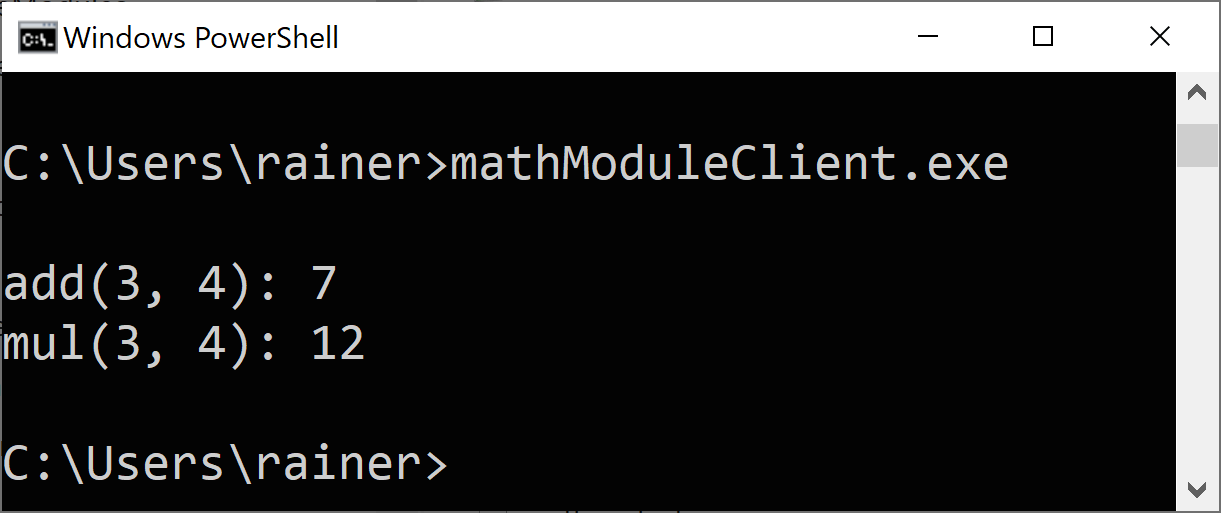
\includegraphics[width=0.6\textwidth]{content/3/chapter4/images/21.png}\\
The usage of function modules and submodules
\end{center}

\begin{tcolorbox}[colback=blue!5!white,colframe=blue!75!black,title=Building the Executable with the Microsoft Compiler]
	
\hspace*{\fill} \\ %插入空行
\noindent
Building the executable out of the modules and its submodules
\begin{tcblisting}{commandshell={}}
cl.exe /c /experimental:module mathModule1.ixx /EHsc
cl.exe /c /experimental:module mathModule2.ixx /EHsc
cl.exe /c /experimental:module mathModule.ixx /EHsc
cl.exe /EHsc /experimental:module mathModuleClient.cpp \
  mathModule1.obj mathModule2.obj mathModule.obj
\end{tcblisting}

Each compilation process of the three modules creates two artifacts: The IFC file (interface file) *.ifc, which is implicitly used in the last line, and the *.obj file, which is explicitly used in the last line.

\end{tcolorbox}

I already mentioned that a submodule is also a module. Each submodule has a module declaration. Consequently, I can create a second client that is only interested in the math.math1 module.

\hspace*{\fill} \\ %插入空行
\noindent
The main program uses only submodule math.math1
\begin{lstlisting}[style=styleCXX]
// mathModuleClient1.cpp
#include <iostream>
import math.math1;
int main() {
	std::cout << '\n';
	std::cout << "add(3, 4): " << add(3, 4) << '\n';
}
\end{lstlisting}

\begin{center}
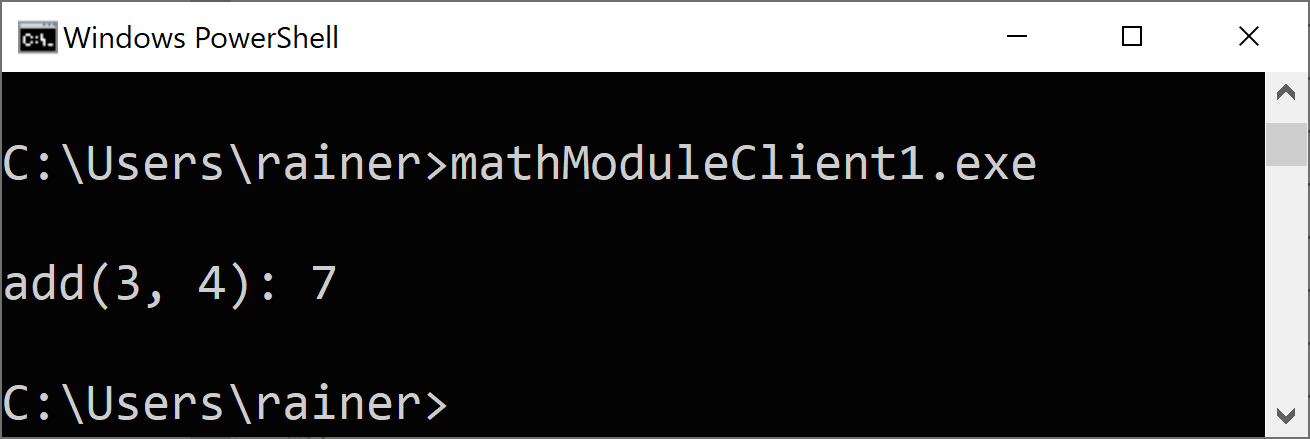
\includegraphics[width=0.6\textwidth]{content/3/chapter4/images/22.png}\\
The usage of function modules and submodules
\end{center}

The division of modules into modules and submodules is a means for the module designer to give the user of the module the possibility to import fine-grained parts of the module. This observation does not apply to module partitions.

\hspace*{\fill} \\ %插入空行
\noindent
4.2.8.2\hspace{0.2cm} Module Partitions

A module can be divided into partitions. Each partition consists of a module interface unit (partition interface file) and zero or more module implementation units (see Module Interface Unit and Module Implementation Unit). The names that the partitions export are imported and re-exported by the primary module interface unit (primary interface file). The names of a partition must begin with the name of the module. The partitions cannot exist on their own.

The description of module partitions is more difficult to understand than its implementation. In the following lines, I rewrite the math module and its submodules math.math1 and math.math2 (see Submodules) to module partitions. In this straightforward process, I refer to the shortly introduced terms of module partitions.

\hspace*{\fill} \\ %插入空行
\noindent
Primary interface file
\begin{lstlisting}[style=styleCXX]
// mathPartition.ixx

export module math;

export import :math1;
export import :math2;
\end{lstlisting}

The primary interface file consists of the module declaration (line 3). It imports and re-exports the partitions math1 and math2 using colons (lines 5 and 6). The name of the partitions must begin with the name of the module. Consequently, you don’t have to specify them.

\hspace*{\fill} \\ %插入空行
\noindent
First module partition
\begin{lstlisting}[style=styleCXX]
// mathPartition1.ixx

export module math:math1;

export int add(int fir, int sec) {
	return fir + sec;
}
\end{lstlisting}

\hspace*{\fill} \\ %插入空行
\noindent
Second module partition
\begin{lstlisting}[style=styleCXX]
// mathPartition2.ixx

export module math:math2;

export {
	int mul(int fir, int sec) {
		return fir * sec;
	}
}
\end{lstlisting}

Similar to the module declaration, the expressions export module math:math1 and export module math:math2 (line 3) declare a module interface partition. A module interface partition is also a module interface unit. The name math stands for the module and the names math1 or math2 for the partition.

\hspace*{\fill} \\ %插入空行
\noindent
Import the module partition
\begin{lstlisting}[style=styleCXX]
// mathModuleClient.cpp
import math;
int main() {
	std::cout << '\n';
	std::cout << "add(3, 4): " << add(3, 4) << '\n';
	std::cout << "mul(3, 4): " << mul(3, 4) << '\n';
}
\end{lstlisting}

You may have already assumed it: The client program is identical to the client program I previously used with submodules. The same observation holds for the creation of the executable and the execution of the program:

\begin{center}
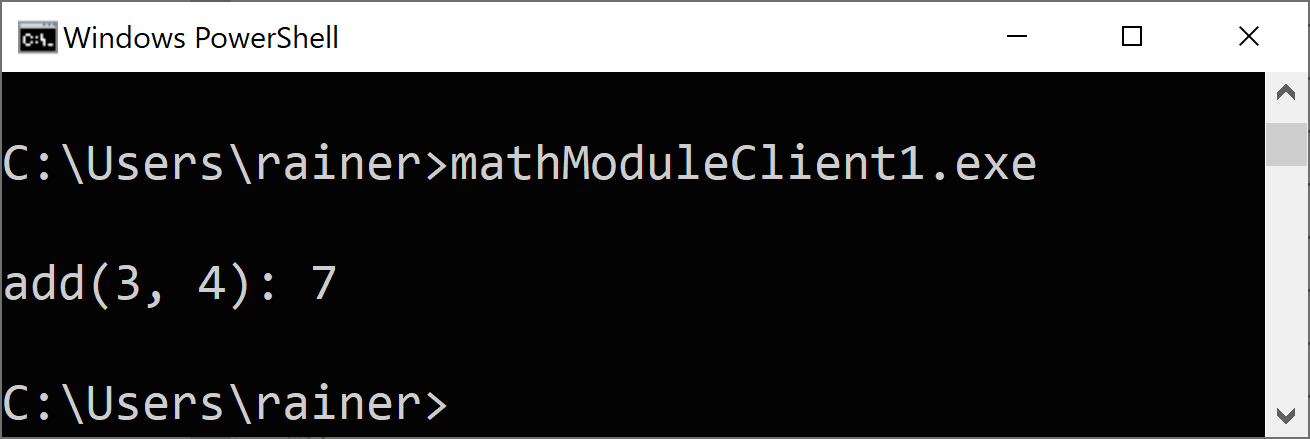
\includegraphics[width=0.6\textwidth]{content/3/chapter4/images/23.png}\\
The usage of function modules and submodules
\end{center}

\subsubsubsection{4.2.9\hspace{0.2cm} Templates in Modules}

I often hear the question: How are templates exported by modules? When you instantiate a template, its definition must be available. This is the reason that template definitions are hosted in headers. Conceptually, the usage of a template has the following structure

\hspace*{\fill} \\ %插入空行
\noindent
4.2.9.1\hspace{0.2cm} Without Modules

\begin{itemize}
\item 
templateSum.h

\noindent
Definition of the function template sum
\begin{lstlisting}[style=styleCXX]
// templateSum.h
template <typename T, typename T2>
auto sum(T fir, T2 sec) {
	return fir + sec;
}
\end{lstlisting}

\item 
sumMain.cpp

\noindent
Use of the template sum
\begin{lstlisting}[style=styleCXX]
// sumMain.cpp
#include <templateSum.h>
int main() {
	sum(1, 1.5);
}
\end{lstlisting}
\end{itemize}

The main program directly includes the header templateSum.h. The call sum(1, 1.5) triggers the template instantiation. In this case, the compiler generates out of the function template sum the concrete function sum, which takes an int and a double as arguments. If you want to visualize this process, use the example on \href{https://cppinsights.io/}{C++ Insights}.

\hspace*{\fill} \\ %插入空行
\noindent
4.2.9.2\hspace{0.2cm} With Modules

With C++20, templates can and should be in modules. Modules have a unique internal representation that is neither source code nor assembly. This representation is a kind of an \href{https://en.wikipedia.org/wiki/Abstract_syntax_tree}{abstract syntax tree} (AST). Thanks to this AST, the template definition is available during template instantiation.

In the following example, I define the function template sum in module math.

\begin{itemize}
\item 
mathModuleTemplate.ixx

\noindent
Definition of the function template sum
\begin{lstlisting}[style=styleCXX]
// mathModuleTemplate.ixx
export module math;
export namespace math {
	template <typename T, typename T2>
	auto sum(T fir, T2 sec) {
		return fir + sec;
	}
}
\end{lstlisting}

\item 
clientTemplate.cpp

\noindent
Use of the function template sum
\begin{lstlisting}[style=styleCXX]
// clientTemplate.cpp
#include <iostream>
import math;
int main() {
	std::cout << '\n';
	std::cout << "math::sum(2000, 11): " << math::sum(2000, 11) << '\n';
	std::cout << "math::sum(2013.5, 0.5): " << math::sum(2013.5, 0.5) << '\n';
	std::cout << "math::sum(2017, false): " << math::sum(2017, false) << '\n';
}
\end{lstlisting}
\end{itemize}

The command line to compile the program is not different from the previous ones. Consequently, I skip it and present the output of the program directly:

\begin{center}
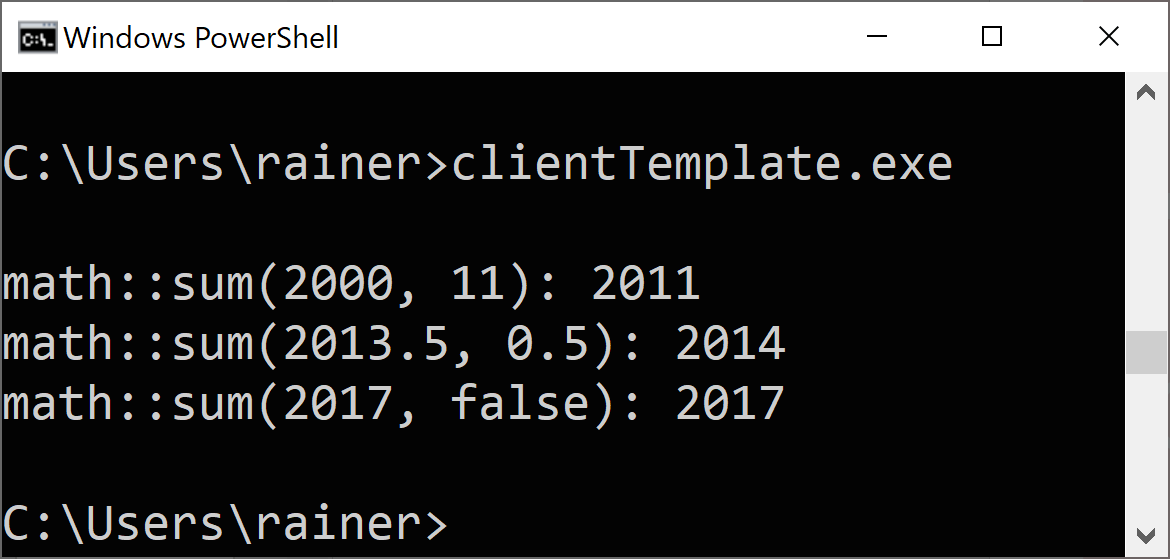
\includegraphics[width=0.6\textwidth]{content/3/chapter4/images/24.png}\\
Use of the function template sum
\end{center}

With modules, we get a new kind of linkage.

\subsubsubsection{4.2.10\hspace{0.2cm} Module Linkage}

Until C++20, C++ supported two kinds of linkage: internal linkage and external linkage.

\begin{itemize}
\item 
Internal linkage: Names with internal linkage are not accessible outside the translation unit. Internal linkage includes mainly namespace-scope names that are declared static and members of anonymous namespaces.

\item 
Internal linkage: Names with internal linkage are not accessible outside the translation unit. Internal linkage includes mainly namespace-scope names that are declared static and members of anonymous namespaces.
\end{itemize}

Modules introduce module linkage:

\begin{itemize}
\item 
Module linkage: Names with module linkage are only accessible inside the module. Names have module linkage if they don’t have external linkage and they are not exported.
\end{itemize}

A small variation of the previous module declaration mathModuleTemplate.ixx makes my point. Imagine that I want to return to the user of my function template sum not only the result of the addition, but also the return type the compiler deduces.

\hspace*{\fill} \\ %插入空行
\noindent
An improved definition of the function template sum
\begin{lstlisting}[style=styleCXX]
// mathModuleTemplate1.ixx

module;

#include <iostream>
#include <typeinfo>
#include <utility>

export module math;

emplate <typename T>
auto showType(T&& t) {
	return typeid(std::forward<T>(t)).name();
}

export namespace math {

	template <typename T, typename T2>
	auto sum(T fir, T2 sec) {
		auto res = fir + sec;
		return std::make_pair(res, showType(res));
	}

}
\end{lstlisting}

nstead of the sum of the numbers, the function template sum returns a \href{https://en.cppreference.com/w/cpp/utility/pair}{std::pair} (line 21) consisting of the sum and a string representation of the type of the value res. Note that I put the function template showType (line 11) outside the exported namespace math (line 16). Consequently, invoking it from outside the module math is not possible. Function template showType uses \href{https://www.modernescpp.com/index.php/perfect-forwarding}{perfect forwarding} to preserve the value categories of the function argument t. The \href{https://en.cppreference.com/w/cpp/language/typeid}{typeid} operator queries information about the type at run time (\href{https://en.cppreference.com/w/cpp/types}{run time type identification (RTTI)}).

\hspace*{\fill} \\ %插入空行
\noindent
Use of the improved function template sum
\begin{lstlisting}[style=styleCXX]
// clientTemplate1.cpp

#include <iostream>
import math;

int main() {
	
	std::cout << '\n';
	
	auto [val, message] = math::sum(2000, 11);
	std::cout << "math::sum(2000, 11): " << val << "; type: " << message << '\n';
	
	auto [val1, message1] = math::sum(2013.5, 0.5);
	std::cout << "math::sum(2013.5, 0.5): " << val1 << "; type: " << message1
			  << '\n';
	auto [val2, message2] = math::sum(2017, false);
	std::cout << "math::sum(2017, false): " << val2 << "; type: " << message2
			  << '\n';

}
\end{lstlisting}

Now, the program displays the value of the summation and a string representation of the automatically deduced type.

\begin{center}
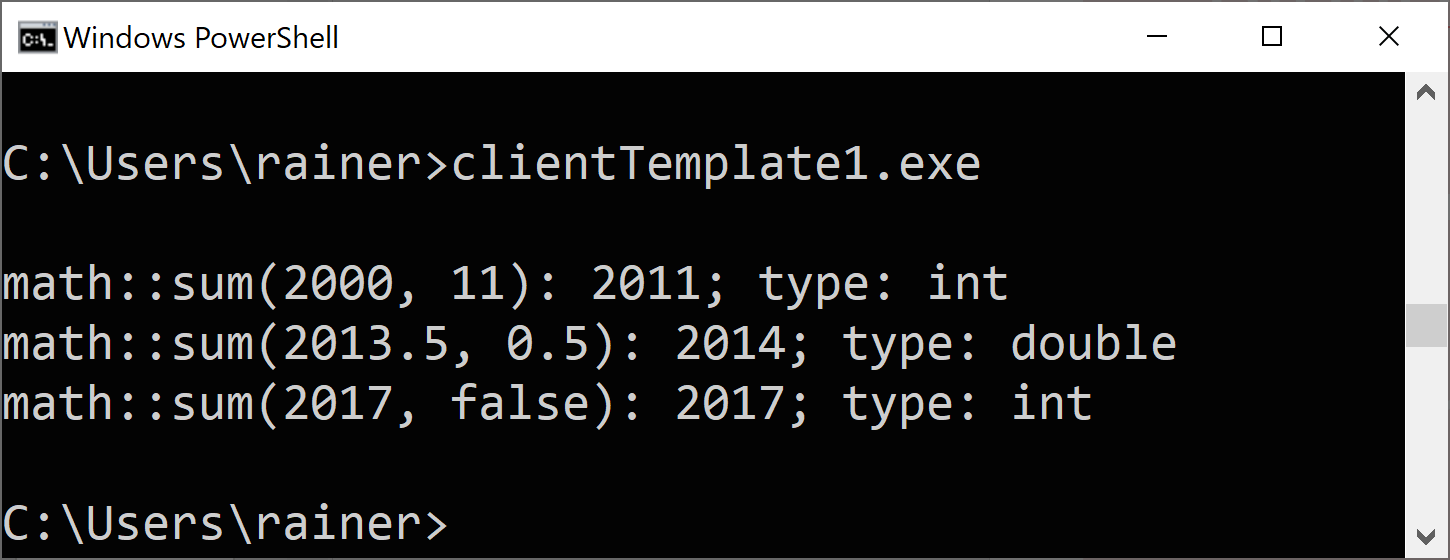
\includegraphics[width=0.8\textwidth]{content/3/chapter4/images/25.png}\\
Use of the improved function template sum
\end{center}

\subsubsubsection{4.2.11\hspace{0.2cm} Header Units}

At the end of 2020, no compiler, so far, supports header units. Header units are a smooth way to transition from headers to modules. You just have to replace the \#include directive with the new import directive.

\hspace*{\fill} \\ %插入空行
\noindent
Replacing \#include directives with import directives
\begin{lstlisting}[style=styleCXX]
#include <vector> => import <vector>;
#include "myHeader.h" => import "myHeader.h";
\end{lstlisting}

First, import respects the same lookup rules as include. This means in the case of the quotes ("myHeader.h") that the lookup first searches in the local directory before it continues with the system search path.

Second, this is way more than text replacement. In this case, the compiler generates something module-like out of the import directive and treats the result as if it would be a module. The importing module statement gets all exportable names from the header. The exported names include macros. Importing these synthesized header units is faster than including header files and comparable in speed to precompiled headers.

\hspace*{\fill} \\ %插入空行
\noindent
4.2.11.1\hspace{0.2cm} One Drawback

There is one drawback with header units. Not all headers are importable. Which headers are importable is \href{https://en.cppreference.com/w/cpp/language/ub}{implementation-defined}, but the C++ standard guarantees that all standard library headers are importable headers. The ability to import excludes C headers. They are just wrapped in the std namespace. For example <cstring> is the C++ wrapper for <string.h>. You can easily identify the wrapped C header because the pattern is: xxx.h gets cxxx.

\begin{tcolorbox}[colback=mygreen!5!white,colframe=mygreen!75!black,title=Building the Executable with the Microsoft Compiler]

\begin{itemize}
\item 
Modules overcome the deficiencies of headers and macros, in particular. Their import is literally for free, and in contrast to macros, the sequence in which you import does not matter. Additionally, they overcome name collisions.

\item 
A module consists of a module interface unit and a module implementation unit. There must be one module interface unit having the exporting module declaration and arbitrarily many module implementation units. Names that are not exported in the module interface have module linkage and cannot be used outside the module.

\item 
Modules can have headers or import and re-export other modules.

\item 
The standard library in C++20 is not modularized. Building your modules is with C++20 a challenging task.

\item 
To structure large software systems, modules provide two ways: submodules and partitions. In contrast to a partition, a submodule can live on its own.

\item 
Thanks to header units, you can replace an include statement with an import statement, and the compiler autogenerates a module.
\end{itemize}

\end{tcolorbox}











































